% **************************************************************
% Hi! Edit this file for your presentation!
% **************************************************************

% ==================///==================///==================///
% ==================/// LATEX'S STUFF
% ==================///==================///==================///

\documentclass{beamer}
%----------------------Packages--------------------------------
\usepackage{amsfonts,amsmath,oldgerm}
\usepackage{listings}
\usepackage{colortbl}
\usepackage{listings}
\usetheme{_statale}
\usefonttheme[onlymath]{serif}
\usepackage[style=verbose,backend=bibtex]{biblatex}
\addbibresource{references.bib} % Your bibliography file
%----------------------our packages------------------------------
\usepackage[utf8]{inputenc}
\usepackage{hyperref}
\usepackage{amsmath}
\usepackage{centernot}
\usepackage{algpseudocode}
\usepackage{algorithm}
\usepackage[T1]{fontenc}
\usepackage{libertine}
\usepackage{pifont}
\usepackage{tikz}
\usepackage{enumitem}
\usetikzlibrary{shapes.misc, positioning}
% Define colors for text
\definecolor{TextRed}{RGB}{255, 0, 0}
\definecolor{TextGreen}{RGB}{0, 255, 0}

\definecolor{AlertRed}{RGB}{255, 0, 0}
\definecolor{TextTeal}{RGB}{0, 128, 128}
\usetikzlibrary{shapes.geometric, arrows, positioning}
\usepackage{mwe}% for example pictures
\usepackage{latexsym,xcolor,multicol,booktabs,calligra}
\usepackage{amsmath,amssymb,BOONDOX-cal,bm}	
\usepackage{graphicx,pstricks,stackengine} 
\usepackage{multicol,multirow}
\usetikzlibrary{matrix,decorations.pathreplacing,calc}
\usepackage[dvipsnames]{xcolor}
% \usepackage{tcolorbox}

%--------------------User defined shapes--------------------------
\tikzstyle{startstop} = [ellipse, minimum width=0.4cm, minimum height=0.125cm, text centered, draw=white, text = teal]
\tikzstyle{io} = [trapezium, trapezium left angle=70, trapezium right angle=110, minimum width=0.5cm, minimum height=0.15cm, text centered, draw=white, text = teal]
\tikzstyle{process} = [rectangle, minimum width=0.5cm, minimum height=0.15cm,text centered, text = teal, draw=white]
\tikzstyle{decision} = [diamond, minimum width=0.3cm, minimum height=0.15cm, text centered, draw=white, text = teal, scale=0.4]
\tikzstyle{arrow} = [thick,->,>=stealth]
\setbeamercolor{finalblock}{bg=green!30, fg=black} % Background and text color for final answer block

\newenvironment{finalanswer}{\begin{block}{Final Answer}}{\end{block}} % Define a custom environment for the final answer block
%---------------------User defined colors---------------------
\definecolor{deeppurple}{RGB}{102, 0, 153}
%--------------------template code--------------------------------
\setbeamertemplate{caption}[numbered]
\newcommand{\testcolor}[1]{\colorbox{#1}{\textcolor{#1}{test}}~\texttt{#1}}
\newcommand{\hrefcol}[2]{\textcolor{frmtxt}{\href{#1}{#2}}}
\titlebackground*{assets/background}

% ==================///==================///==================///
% ==================/// SPLASH PAGE
% ==================///==================///==================///

\title{\textsc{Lempel-Ziv-Welch}}
\subtitle{Compression Algorithm}
\institute[CSE,BUET]
{
  Department of Computer Science and Engineering\\
  Bangladesh University of Engineering and Technology
}
\author[Munim,Tabib,Tias]{2005097:Munim Thahmid \\ 2005103:H.M.Shadman Tabib \\ 2005106:Tasriad Ahmed Tias}
\date{\today}


% ==================///==================///==================///
% ==================/// START PRESENTATION
% ==================///==================///==================///
%-----------------template codde---------------------------------
\pgfplotsset{compat=1.18}
\usetikzlibrary{positioning}
\begin{document}
\maketitle

% \begingroup
%     \setbeamertemplate{frametitle}{%
%       \vspace*{-3.5ex}
%       \begin{beamercolorbox}[leftskip = 2cm]{frametitle}%
%         \usebeamerfont{frametitle}\insertframetitle\\
%       \end{beamercolorbox}
%     }
%     \themecolor{main}
%     \begin{frame}{Table of Contents}
%        \tableofcontents
%     \end{frame}
% \endgroup


% ==================///==================///==================///
% ==================/// BODY'S PRESENTATION
% ==================///==================///==================///

%-----------------------Tias-------------------------------------
\section{Introduction}
\begin{frame}{Comparison between compressed and uncompressed files}
\centering
    \begin{table}[h]
    \caption{Uncompressed file size vs Compressed file size}
    \begin{tabular}{| C | c | c | C |}
    \hline
       Files: & \includegraphics[width=0.1\textwidth, height=0.1\textwidth]{assets/video_logo.png} &
        \includegraphics[width=0.1\textwidth, height=0.1\textwidth]{assets/image_logo.png} & \includegraphics[width=0.1\textwidth, height=0.1\textwidth]{assets/pdf_file_logo.png}\\
        \hline
        Length: & 1 minute & 24-bit color & 1 page \\
        \hline
        Uncompressed Size: & 2 GB & 500 MB & 10 MB \\
        \hline
        Compressed Size: & 5-10 MB & 1 MB & 10 KB \\
        \hline
    \end{tabular}
    \begin{tabular}{c c c c}
        \includegraphics[width=0.08\textwidth, height=0.08\textwidth]{assets/think.png} & \multicolumn{3}{c}{\textbf{Huge Difference!}} \\
          
    \end{tabular}
\end{table}
\end{frame}

\begin{frame}{Why need Compression?}
 \begin{itemize}
     \item If the file size of a 1-minute video is 2 GB, what would the size of a 2-hour-long movie be?
     \item \includegraphics[width=0.4\textwidth, height=0.3\textwidth]{assets/surprised.png}
 \end{itemize}
\end{frame}

\begin{frame}{Intro to LZW}
    \begin{itemize}[label=$\blacksquare$]
        \item This is where compression algorithms come into the picture. \\
        \item \textsc{Lempel–Ziv–Welch} (LZW) is a universal lossless data compression algorithm created by Abraham Lempel, Jacob Ziv, and Terry Welch.
        \item As a lossless compression algorithm the core idea is to reduce bits by identifying and eliminating statistical redundancy.
        \item Also there will be no loss of data after compression.
    \end{itemize}
\end{frame}

\section{Understanding LZW}
\begin{frame}{How does it work?}
\begin{itemize}[label=\ding{79}]
\color{orange}
    \item <1->LZW compression works by reading a sequence of symbols, grouping the symbols into strings, and converting the strings into codes.
    \item <2-> Since codes take up less space than the strings they replace, we get compression.
    \item <3-> In other words, this algorithm scans a file for data patterns that appear more than once. These patterns are then saved in a dictionary, and references are placed within the compressed file wherever repetitive data occurs.
\end{itemize}
\end{frame}

\begin{frame}{Flowchart}
\centering
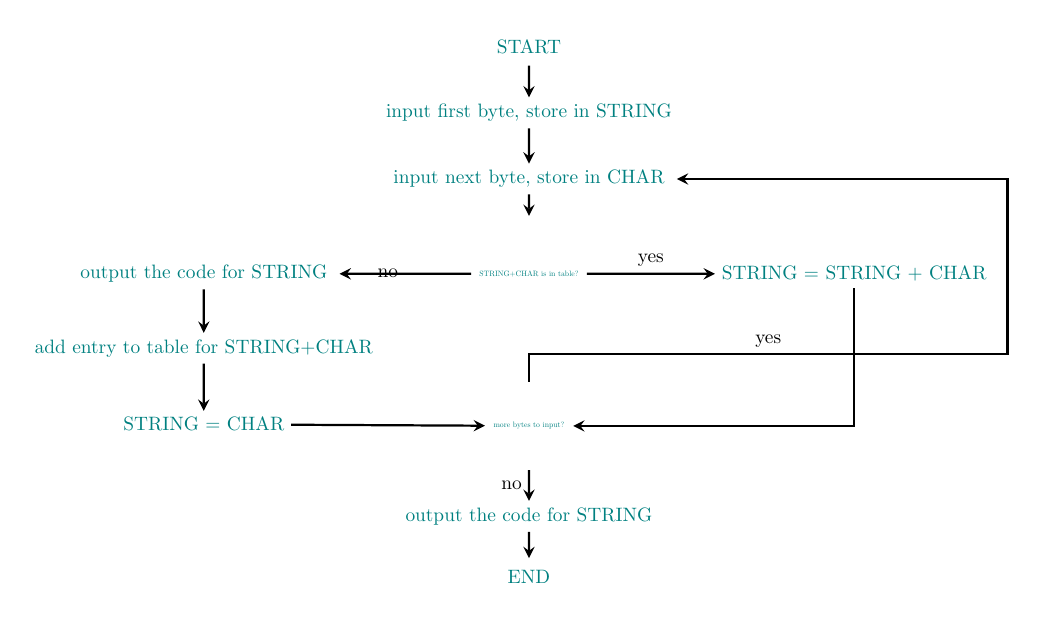
\begin{tikzpicture}[node distance=0.9cm, scale=0.7, every node/.style={scale=0.7}]
\node (start) [startstop] {START};
\node (in1) [io, below of=start, yshift=-0.3cm] {input first byte, store in STRING};
\node (in2) [io, below of=in1, yshift=-0.3cm] {input next byte, store in CHAR};
\node (dec1) [decision, below of=in2, yshift= -3.4cm] {STRING+CHAR is in table?};
\node (pro1) [io, left of=dec1, xshift=-5cm] {output the code for STRING};
\node (pro2) [process, below of=pro1,yshift=-0.45cm] {add entry to table for STRING+CHAR};
\node (pro3) [process, below of=pro2,yshift=-0.48cm] {STRING = CHAR};
\node (pro4) [process, right of=dec1, xshift=5cm] {STRING = STRING + CHAR};
\node (dec2) [decision, below of=dec1, yshift=-6cm] {more bytes to input?};
\node (pro5) [process, below of=dec1, yshift=-3.5cm] {output the code for STRING};
\node (stop) [startstop, below of=pro5, yshift=-0.2cm] {END};

\draw [arrow] (start) -- (in1);
\draw [arrow] (in1) -- (in2);
\draw [arrow] (in2) -- (dec1);
\draw [arrow] (dec1) -- node[anchor=east] {no} (pro1);
\draw [arrow] (pro1) -- (pro2);
\draw [arrow] (pro2) -- (pro3);
\draw [arrow] (pro3) -- (dec2);
\draw [arrow] (dec1) -- node[anchor=south] {yes} (pro4);
\draw [arrow] (pro4) |- (dec2);
\draw [arrow] (dec2) -- node[anchor=east] {no} (pro5);
\draw [arrow] (pro5) -- (stop);
\draw [arrow] (dec2.north) -- ++(0,0.5) -| node[near start, above] {yes} ([xshift=6cm]in2.east) -- (in2.east);

\end{tikzpicture}
    
\end{frame}

\begin{frame}{Pseudocode}
    \begin{figure}
        \centering
        \includegraphics[scale = 0.5]{assets/encoding_pseudocode.png}
        \caption{Pseudocode for Encoding}
        \label{fig:enter-label}
    \end{figure}
\end{frame}
\section{Example: Compression Process}
\begin{frame}{Uncompressed ASCII String}
        \textcolor{cyan}{
        I want to compress the following string: \\
    }
    \textcolor{yellow}{
        \begin{center}
             \textbf{\large thisisthe} \\  
        \end{center}
    }
    \textcolor{cyan}{
        By default using uncompressed ASCII, this is equal to: \\
    }
        0111010 \;0110100 \;0110100 \;0111001 \;0111001 \;0111010 \;0110100 \;0110101 \;0111011 \\
        \quad116 \quad\quad104 \quad\quad\:105 \quad\quad\;115 \quad\quad\;105 \quad\quad115 \quad\quad\:116 \quad\quad\;104 \quad\quad101\\
    \textcolor{cyan}{That's 72 bits. We can do better!}\\
    \begin{center}
        \includegraphics[scale=0.2]{assets/motivated.png}
    \end{center}
\end{frame}
\begin{frame}{Compression Process}
    \begin{itemize}[label=\ding{60}]
    \color{olive}
        \item ASCII values are of 8 bits. The idea is to extend it from 9 to 12 bits to identify recurring subsections. 
    \end{itemize}
\end{frame}
\begin{frame}{Compression Process}
    \textcolor{cyan}{
        I want to compress the following string: \\
        \begin{center}
        \textcolor{yellow}{
        \textbf{\large thisisthe}
        }
        \end{center}
    }    
    \begin{itemize}[label=\ding{118}]
        \color{lime}
        \item <1->Start adding pairs of symbols to a dictionary of words.
        \item <2-> When we reach a pair that we've already placed in the dictionary, replace that pair with our new dictionary value.
        \item <3-> For this tiny string, we will only need 9 bits, allowing up to 512 unique symbols.
    \end{itemize}
\end{frame}
\begin{frame}{Example: Lempel Ziv Welch Algorithm}
\textcolor{cyan}{
I want to compress the following string: \\
}
\begin{center}
    \textcolor{yellow}{\textbf{\large thisisthe}}
\end{center}
\begin{itemize}
    \item <1-> \quad\quad Current \quad\quad\quad\quad Next \quad\quad\quad\quad Output \quad\quad\quad\quad Add to dictionary
    \item <1-> \quad\quad \textcolor{yellow}{t}\:\textcolor{cyan}{116} \quad\quad\quad\qquad\: \textcolor{yellow}{h}\:\textcolor{cyan}{104} \quad\quad\qquad \textcolor{yellow}{t}\:\textcolor{cyan}{116} \quad\quad\quad\qquad\: \textcolor{yellow}{th}\:\textcolor{cyan}{256}
    \item <2-> \quad\quad \textcolor{yellow}{h}\:\textcolor{cyan}{104} \quad\quad\quad\qquad\, \textcolor{yellow}{i}\:\textcolor{cyan}{105} \quad\quad\qquad \textcolor{yellow}{h}\:\textcolor{cyan}{104} \quad\quad\quad\qquad\: \textcolor{yellow}{hi}\:\textcolor{cyan}{257}
    \item <3-> \quad\quad \textcolor{yellow}{i}\:\textcolor{cyan}{105} \quad\quad\quad\qquad\;\, \textcolor{yellow}{s}\:\textcolor{cyan}{115} \quad\quad\qquad \textcolor{yellow}{i}\:\textcolor{cyan}{105} \quad\quad\quad\qquad\; \textcolor{yellow}{is}\:\textcolor{cyan}{258}
    \item <4-> \quad\quad \textcolor{yellow}{s}\:\textcolor{cyan}{115} \quad\quad\quad\qquad\; \textcolor{yellow}{i}\:\textcolor{cyan}{105} \quad\quad\qquad \textcolor{yellow}{s}\:\textcolor{cyan}{115} \quad\quad\quad\qquad\: \textcolor{yellow}{si}\:\textcolor{cyan}{259}
    \item <5-> \quad\quad \textcolor{yellow}{i}\:\textcolor{cyan}{116} \quad\quad\quad\qquad\;\, \textcolor{yellow}{s}\:\textcolor{cyan}{104} \quad\quad\qquad \textcolor{yellow}{"is" is in the dictionary! Check if "ist" is.}
    \item <6-> \quad\quad \textcolor{yellow}{is}\:\textcolor{cyan}{258} \quad\quad\quad\qquad\, \textcolor{yellow}{t}\:\textcolor{cyan}{116} \quad\quad\qquad \textcolor{yellow}{is}\:\textcolor{cyan}{258} \quad\quad\quad\qquad \textcolor{yellow}{ist}\:\textcolor{cyan}{260}
    \item <7-> \quad\quad \textcolor{yellow}{t}\:\textcolor{cyan}{116} \quad\quad\quad\qquad\; \textcolor{yellow}{h}\:\textcolor{cyan}{104} \quad\quad\qquad \textcolor{yellow}{"th" is in the dictionary! Check if "the" is.}    
    \item <8-> \quad\quad \textcolor{yellow}{th}\:\textcolor{cyan}{256} \quad\quad\quad\qquad \textcolor{yellow}{e}\:\textcolor{cyan}{101} \quad\quad\qquad \textcolor{yellow}{th}\:\textcolor{cyan}{256} \quad\quad\quad\qquad \textcolor{yellow}{the}\:\textcolor{cyan}{261}
    \item <9-> \quad\quad \textcolor{yellow}{e}\:\textcolor{cyan}{101} \quad\quad\quad\qquad\: \textcolor{yellow}{-}\:\textcolor{cyan}{-} \quad\qquad\qquad \textcolor{yellow}{e}\:\textcolor{cyan}{101} \quad\quad\quad\qquad\: \textcolor{yellow}{-}\:\textcolor{cyan}{-}
\end{itemize}
\end{frame}
\begin{frame}{Example: Lempel Ziv Welch Algorithm}
    \includegraphics[scale=0.5]{assets/bypass.png}
\end{frame}
\begin{frame}{Example: Lempel Ziv Welch Algorithm}
        \textcolor{cyan}{
        I want to compress the following string: \\
    }
    \textcolor{yellow}{
        \begin{center}
             \textbf{\large thisisthe} \\  
        \end{center}
    }
    \textcolor{cyan}{
        By LZW using compressed ASCII, this is equal to: \\
    }
        0110100 \;0110101 \;01110011 \;0110101 \;01110011 \;01110100 \\
        \quad116 \quad\quad104 \quad\quad\;105 \quad\quad\;115 \qquad\: 258 \qquad\; 256 \\
    \textcolor{cyan}{That's 63 bits instead of the original 72 bits.}\\
    \textcolor{cyan}{That's 87.5\% of what it used to be!}\\
    \begin{columns}
        \column{0.6\linewidth}
        % Text column
        % Empty column to push the image to the right
        \column{0.2\linewidth}
        \hfill
        % Image column
        \includegraphics[scale=0.4]{assets/thumbs_up.png}
    \end{columns}
\end{frame}
%--------------------------Tabib---------------------------------
\section{Advantages of LZW}

\begin{frame}{FACTS about the LZW Algorithm}
    \begin{itemize}
        \item<1-> \textcolor{TextTeal}{\textbf{Efficient Compression:}} LZW provides good compression ratios\footfullcite{lzw1984}, especially for files with repetitive content, by creating a dictionary of substrings as it reads through the data.
        \item<2-> \textcolor{TextTeal}{\textbf{No Prior Knowledge Needed:}} It does not require prior knowledge of the data to compress, as it dynamically builds the dictionary during the compression process.
        \item<3-> \textcolor{TextTeal}{\textbf{Simplicity and Speed:}} The algorithm is simple and fast, with relatively low memory requirements, making it suitable for real-time data compression in various applications.
    \end{itemize}
\end{frame}



\section{Example: Compression Limitations}
% Define the colors for the alert block
\definecolor{alertBlockTitleColor}{RGB}{255,255,255} % white
\definecolor{alertBlockBodyColor}{RGB}{255,255,255} % white
\definecolor{alertBlockBorderColor}{RGB}{255,0,0} % red

\setbeamercolor{block title alerted}{fg=alertBlockTitleColor,bg=alertBlockBorderColor}
\setbeamercolor{block body alerted}{fg=alertBlockBodyColor,bg=alertBlockBorderColor}

\setbeamertemplate{blocks}[rounded][shadow=true]


\begin{frame}{Example: Compression Limitations}
    \begin{alertblock}{}
        \centering
        \textbf{\textit{"Does Compression Algorithm always Compress?"}}
    \end{alertblock}
\end{frame}
\begin{frame}[fragile]{LZW Compression Table}
\begin{figure}
\centering
\includegraphics[width=\textwidth]{assets/1.png}
\end{figure}
\end{frame}
\begin{frame}[fragile]{LZW Compression Table}
\begin{figure}
\centering
\includegraphics[width=\textwidth]{assets/2.png}
\end{figure}
\end{frame}
\begin{frame}[fragile]{LZW Compression Table}
\begin{figure}
\centering
\includegraphics[width=\textwidth]{assets/3.png}
\end{figure}
\end{frame}
\begin{frame}[fragile]{LZW Compression Table}
\begin{figure}
\centering
\includegraphics[width=\textwidth]{assets/4.png}
\end{figure}
\end{frame}
\begin{frame}[fragile]{LZW Compression Table}
\begin{figure}
\centering
\includegraphics[width=\textwidth]{assets/5.png}
\end{figure}
\end{frame}
\begin{frame}[fragile]{LZW Compression Table}
\begin{figure}
\centering
\includegraphics[width=\textwidth]{assets/6.png}
\end{figure}
\end{frame}
\begin{frame}[fragile]{LZW Compression Table}
\begin{figure}
\centering
\includegraphics[width=\textwidth]{assets/7.png}
\end{figure}
\end{frame}
\begin{frame}[fragile]{LZW Compression Table}
\begin{figure}
\centering
\includegraphics[width=\textwidth]{assets/8.png}
\end{figure}
\end{frame}
\begin{frame}[fragile]{LZW Compression Table}
\begin{figure}
\centering
\includegraphics[width=\textwidth]{assets/9.png}
\end{figure}
\end{frame}
\begin{frame}[fragile]{LZW Compression Table}
\begin{figure}
\centering
\includegraphics[width=\textwidth]{assets/10.png}
\end{figure}
\end{frame}

\begin{frame}
    \frametitle{LET'S HAVE A LOOK}
    \begin{figure}
        \centering
        \begin{minipage}[c]{0.4\textwidth}
            \includegraphics[scale=0.4]{assets/face-palm.png} % Replace with the path to your first image
        \end{minipage}
        \hfill
        \begin{minipage}[c]{0.4\textwidth}
        \quad\quad\quad
            \includegraphics[scale=0.25]{assets/thunder.png} % Replace with the path to your second image
        \end{minipage}
    \end{figure}

    % Display the alert text
    \begin{center}
        \textcolor{AlertRed}{\Large SOMETHING WRONG!!}
    \end{center}
\end{frame}
\begin{frame}{FACTS ...........}
    \begin{itemize}
        \item<1-> \textcolor{TextRed}{\textbf{IN THIS CASE THE ENCODED STRING IS LONGER THAN THE INPUT}}
        \item<2-> \textcolor{TextRed}{\textbf{BECAUSE THERE IS NO REDUNDANCIES}}
        \item<3-> \textcolor{TextGreen}{\textbf{IN PRACTICAL CASES WE LOOK BACK AT THE LAST 32KB OF DATA WHERE WE WOULD HAVE A LOT OF REDUNDANCIES}}

    \end{itemize}
\end{frame}
\begin{frame}{Drawback}
  \begin{block}<1->{Conclusion}
    LZW algorithm has potential drawback for smaller and non redundant  data
  \end{block}
\end{frame}
%-------------------------Munim----------------------------------
\section{Decompression Process}

 \begin{frame}{What is Decompression?}
  \begin{block}<1->{Definition}
    Decompression is the process of restoring compressed data to its original form or size.
  \end{block}
  
  \begin{block}<2->{}
    \textcolor{blue}{A reverse process of compression}
  \end{block}
\end{frame}



\begin{frame}{Prerequisites for Decompression}
    \begin{block}{Question}
        What are the prerequisites for decompression?
    \end{block}
    
    \begin{itemize}
        \item[{\color{white}\textbullet}]<1-> Compressed Data
        \item[{\color{white}\textbullet}]<2-> Number of bits used during compression
    \end{itemize}
\end{frame}

\section{An Example Problem}

\begin{frame}{The Problem}
    
    \begin{block}{Problem Statement}
        Given compressed data:
        
        \begin{center}
            \texttt{\textcolor{black}{116} \textcolor{black}{104} \textcolor{black}{105} \textcolor{black}{115} \textcolor{black}{258}}
        \end{center}
        
        Retrieve the original string from it.(Assume 9 bit compression)
    \end{block}
\end{frame}

\begin{frame}{Solution Steps-Trivial}
      \centering
    \only<1>{\begin{tabular}{ll}
    Current  & :   \textcolor{green}{$116$ $\rightarrow$ \textbf{$t$}} \\
    Next  & :   \textcolor{white}{$104$ $\rightarrow$ \textbf{$h$}} \\
    String & : \textcolor{white}{t}
\end{tabular}}
    \only<2>{\begin{tabular}{ll}
    Current  & :   \textcolor{green}{$104$ $\rightarrow$ \textbf{$h$}} \\
    Next  & :   \textcolor{white}{$105$ $\rightarrow$ \textbf{$i$}}   \\
    String & : \textcolor{white}{th}
    
\end{tabular}}
    \only<3>{\begin{tabular}{ll}
    Current  & :   \textcolor{green}{$105$ $\rightarrow$ \textbf{$i$}} \\
    Next  & :   \textcolor{white}{$115$ $\rightarrow$ \textbf{$s$}}   \\
    String & : \textcolor{white}{thi}
    
\end{tabular}}
     \only<4>{\begin{tabular}{ll}
    Current  & :   \textcolor{green}{$115$ $\rightarrow$ \textbf{$s$}} \\
    Next  & :   \textcolor{red}{$258$ $\rightarrow$ \textbf{$???$}} \\
    String & : \textcolor{white}{this}
    
\end{tabular}}
    \begin{itemize}
        \item <1-> \quad\quad Current \quad\quad\quad\quad Next \quad\quad\quad\quad Output \quad\quad\quad\quad Add to dictionary
    \item <1-> \quad\quad \textcolor{yellow}{t}\:\textcolor{cyan}{116} \quad\quad\quad\qquad\: \textcolor{yellow}{h}\:\textcolor{cyan}{104} \quad\quad\qquad \textcolor{yellow}{t}\:\textcolor{cyan}{116} \quad\quad\quad\qquad\: \textcolor{yellow}{th}\:\textcolor{cyan}{256}
    \item <2-> \quad\quad \textcolor{yellow}{h}\:\textcolor{cyan}{104} \quad\quad\quad\qquad\, \textcolor{yellow}{i}\:\textcolor{cyan}{105} \quad\quad\qquad \textcolor{yellow}{h}\:\textcolor{cyan}{104} \quad\quad\quad\qquad\: \textcolor{yellow}{hi}\:\textcolor{cyan}{257}
    \item <3-> \quad\quad \textcolor{yellow}{i}\:\textcolor{cyan}{105} \quad\quad\quad\qquad\;\, \textcolor{yellow}{s}\:\textcolor{cyan}{115} \quad\quad\qquad \textcolor{yellow}{i}\:\textcolor{cyan}{105} \quad\quad\quad\qquad\; \textcolor{yellow}{is}\:\textcolor{cyan}{258}
    \item <4-> \quad\quad \textcolor{yellow}{s}\:\textcolor{cyan}{115} \quad\quad\quad\qquad\; \textcolor{yellow}{is}\:\textcolor{cyan}{258} \quad\quad\qquad \textcolor{red}{???}\:\textcolor{red}{???} \quad\quad\quad\qquad\: \textcolor{red}{??}\:\textcolor{red}{???}


    \end{itemize}
    
\end{frame}
\begin{frame}{Solution Step-Decompression}
   \begin{itemize}
        \item  \quad\quad Current \quad\quad\quad\quad Next \quad\quad\quad\quad Output \quad\quad\quad\quad Add to dictionary
    \item  \quad\quad \textcolor{yellow}{t}\:\textcolor{cyan}{116} \quad\quad\quad\qquad\: \textcolor{yellow}{h}\:\textcolor{cyan}{104} \quad\quad\qquad \textcolor{yellow}{t}\:\textcolor{cyan}{116} \quad\quad\quad\qquad\: \textcolor{yellow}{th}\:\textcolor{cyan}{256}
    \item  \quad\quad \textcolor{yellow}{h}\:\textcolor{cyan}{104} \quad\quad\quad\qquad\, \textcolor{yellow}{i}\:\textcolor{cyan}{105} \quad\quad\qquad \textcolor{yellow}{h}\:\textcolor{cyan}{104} \quad\quad\quad\qquad\: \textcolor{yellow}{hi}\:\textcolor{cyan}{257}
    \item  \quad\quad  \textcolor{green}{i}\:\textcolor{green}{105} \quad\quad\quad\qquad\;\, \textcolor{green}{s}\:\textcolor{green}{115} \quad\quad\qquad \textcolor{green}{i}\:\textcolor{green}{105} \quad\quad\quad\qquad\; \textcolor{green}{is}\:\textcolor{green}{258}
    \item  \quad\quad \textcolor{yellow}{s}\:\textcolor{cyan}{115} \quad\quad\quad\qquad\; \textcolor{yellow}{is}\:\textcolor{cyan}{258} \quad\quad\qquad \textcolor{yellow}{s}\:\textcolor{cyan}{115 105 115} \qquad\: \textcolor{yellow}{si}\:\textcolor{cyan}{259}


    \end{itemize}
    \vspace{3pt}
    \textbf{Now,How to decompress 258!}
    \begin{itemize}
        \item<1->[$\bullet$]  From our dictionary, we can see 258 is constructed from 105 and 115
        \item<2->[$\bullet$]  Hence, we can \textbf{decompress} it to 105 and 115
        \item <2->[$\bullet$] which refers to \textbf{\textcolor{green}{is}}
    \end{itemize}
    
    
\end{frame}
\begin{frame}{Solution Step-Continued}
\begin{tabular}{ll}
 Current  & :   \textcolor{green}{$115$ $\rightarrow$ \textbf{$s$}} \\
    Next  & :   \textcolor{green}{$258$ $\rightarrow$ \textbf{$is$}} \\
    String & : \textcolor{white}{thisis}
    
\end{tabular}
    \begin{itemize}
        \item \quad\quad Current \quad\quad\quad\quad Next \quad\quad\quad\quad Output \quad\quad\quad\quad Add to dictionary
    \item  \quad\quad \textcolor{yellow}{t}\:\textcolor{cyan}{116} \quad\quad\quad\qquad\: \textcolor{yellow}{h}\:\textcolor{cyan}{104} \quad\quad\qquad \textcolor{yellow}{t}\:\textcolor{cyan}{116} \quad\quad\quad\qquad\: \textcolor{yellow}{th}\:\textcolor{cyan}{256}
    \item  \quad\quad \textcolor{yellow}{h}\:\textcolor{cyan}{104} \quad\quad\quad\qquad\, \textcolor{yellow}{i}\:\textcolor{cyan}{105} \quad\quad\qquad \textcolor{yellow}{h}\:\textcolor{cyan}{104} \quad\quad\quad\qquad\: \textcolor{yellow}{hi}\:\textcolor{cyan}{257}
    \item  \quad\quad \textcolor{yellow}{i}\:\textcolor{cyan}{105} \quad\quad\quad\qquad\;\, \textcolor{yellow}{s}\:\textcolor{cyan}{115} \quad\quad\qquad \textcolor{yellow}{i}\:\textcolor{cyan}{105} \quad\quad\quad\qquad\; \textcolor{yellow}{is}\:\textcolor{cyan}{258}
   \item  \quad\quad \textcolor{yellow}{s}\:\textcolor{cyan}{115} \quad\quad\quad\qquad\; \textcolor{yellow}{is}\:\textcolor{cyan}{258} \quad\qquad \textcolor{yellow}{s}\:\textcolor{cyan}{115 105 115} \qquad\: \textcolor{yellow}{si}\:\textcolor{cyan}{259}


    \end{itemize}
    
\end{frame}
\begin{frame}{Solution Step-Answer}
    \begin{finalanswer}
           Retrieved String: \textbf{thisis}

    \end{finalanswer}
\end{frame}
\section{Algorithm}
\begin{frame}{LZW Decompression Algorithm (Part 1)}
    \begin{block}<1->{Initialization}
        \begin{itemize}
            \item Create a dictionary with single-character entries.
        \end{itemize}
    \end{block}
    
    \begin{block}<2->{Decompression}
        \begin{itemize}
            \item Read the compressed data and start with the first code.
            \item Output the corresponding character and prepare to add new dictionary entries.
        \end{itemize}
    \end{block}
\end{frame}

\begin{frame}{LZW Decompression Algorithm (Part 2)}
    \begin{block}<1->{Loop}
        \begin{itemize}
            \item While there are remaining codes:
            \begin{itemize}
                \item Read the next code.
                \item If not in the dictionary, add a new entry.
                \item Output characters based on codes and update the dictionary.
            \end{itemize}
        \end{itemize}
    \end{block}
    
    \begin{block}<2->{Output}
        \begin{itemize}
            \item The output is the decompressed data.
        \end{itemize}
    \end{block}
    
    \begin{block}<3->{End}
        \begin{itemize}
            \item Finish the decompression process.
        \end{itemize}
    \end{block}
\end{frame}
\begin{frame}[fragile]{PseudoCode}
\begin{lstlisting}[language=Python, basicstyle=\small]
function LZWDecompression(compressedData):
    initialize dictionary with single-character entries
    output = ""
    previousCode = null
    while compressedData is not empty:
        code = getNextCode(compressedData)
        if code is not in dictionary:
            entry = dictionary[previousCode] + dictionary[previousCode][0]
        else:
            entry = dictionary[code]
        output += entry
        if previousCode is not null and code is not in dictionary:
            dictionary.add(dictionary[previousCode] + entry[0])
        previousCode = code
    return output
\end{lstlisting}
\end{frame}





\section{Use Case: Practical Application}
\begin{frame}{Use Case: Practical Application}
    \begin{itemize}
        \item[$\bullet$] Text compression in software applications.
        \item[$\bullet$] Transmission of data over networks with limited bandwidth.
        \item[$\bullet$] Storing data efficiently in databases or file systems.
        \item[$\bullet$] Compressing images, audio, and video files to save storage space.
        \item[$\bullet$] Implementing data compression in web servers to optimize page loading times.
    \end{itemize}
\end{frame}
\section{Conclusion}



% ==================///==================///==================///
% ==================/// END PRESENTATION
% ==================///==================///==================///

\backmatter
\end{document}